\documentclass{cta-author}
\usepackage{subfigure}
\newtheorem{theorem}{Theorem}{}
\newtheorem{corollary}{Corollary}{}
\newtheorem{remark}{Remark}{}

\begin{document}

\title{PCA Preprocessing Target Spectorgram for Birds and Drones Classification}

\author{\au{Siyue Zhang$^{1}$}}

\address{\add{1}{School of Engineering, University of Birmingham}
\email{sxz151@student.bham.ac.uk}}

\begin{abstract}
As the growing of the consumer market of personal drones, technologies are needed to monitor drones in the airspace. Radar has been proven to be a suitable tool for the detection and surveillance of the drone.
One of the main obstacles in drone detection is the interference of the birds; since two targets share the same flight level, ground speed, and size.
In this Final Year Project research, the impact of principal component analysis(PCA) on the classification of birds and drones is investigated and demonstrated. The whole project was built and tested on the L band staring radar dataset. Several different algorithm of PCA is implemented first and a classifier is trained based on support vector machine(SVM). The SVM classifier is used to demonstrate the impact of PCA preprocessing on classification. The impact of preprocessing is evaluated by the results such as training time cost, confusion matrix and general accuracy of classification.
Finally, the different performance of PCA preprocessing algorithm is demonstrated and the reason of these result is concluded. It shows that PCA preprocessing can be an efficient way to increase the performance of the classifier when facing the radar spectrogram data.
\end{abstract}

\maketitle

\section{Introduction}\label{sec1}
In recent years, the development of drones has progressed rapidly and continues to evolve. While drones have brought many benefits to industries such as agriculture and environmental monitoring, concerns have been raised about their misuse. 
The use of drones with cameras has raised concerns over personal privacy as they can capture images or videos without consent. This becomes especially concerning when drones fly over private property.
Drones can also be dangerous to the airspace, Operating drones within restricted airspace, such as near airports or government installations, can interfere with manned aircraft operations and create hazardous situations. In 2016, the FAA raised the alarm about drones in the airspace and received over 100 reports of unmanned aircraft flying near other manned aircraft or airports per month.\cite{1} In a word, efficient and economical ways of surveillance the airspace and protecting key areas from drone intruding such as airports are needed. Radar is one of the most efficient technologies to monitor drones, as well as the only capable device that can offer all-weather, continuous surveillance of a certain area of airspace.

Birds as a radar target, are always the main obstacle in drone detection. Birds and drones share the same flying altitude and ground speed. It is hard to tell the difference by simply looking at the 4-D data(Azimuth, Elevation, Range of time) of radar feedback. Birds unlike drones will not cause privacy or environmental issues and birds can be controlled by bird-repellent devices. Therefore one of the main challenges in designing a drone surveillance radar is the classification of birds and drones.

Machine learning and deep learning techniques have been instrumental in solving the problems of classification. The trend of researching the birds and drones classification problem is adopting machine learning or deep learning algorithms with different features of radar data.
There are a few features of radar that can be utilized to classify birds and drones. 
In\cite{2}, researchers utilized physical features such as height and position and trained a decision tree to solve the classification problem.
In 2015, a group of researchers showed the potential of using polarimetric features to distinguish birds and drones.\cite{3} 
In 2020, a group of researchers provided another approach of using the trajectory differences between birds and drones for classification.\cite{4} They evaluate features of trajectories such as curvature and turning angle, and then train SVM to distinguish these features. 
Another class of related work use visual methods for classification, for instance, in \cite{5}, the researchers classified the birds and drones by training a convolutional neural network (CNN) based on VGG-16 architecture. 

Despite all of the methods with different features above, a trending, as well as popular way, is training the classifier based on the micro-Doppler(u-Doppler) signature. Micro-Doppler is a phenomenon where small, rapid movements of objects within a larger, primary movement generate additional frequency shifts in the radar signal. In the case of drones, the fast rotating blades produce the u-Doppler effect and will produce the Helicopter Rotor Modulation(HERM) lines on the spectrogram of drone target. As for the birds, the flapping of wings can also produce the u-Doppler effect however the frequency of flapping is nothing compared to the rotation of the drone's blade.\cite{6} HERM lines can be discovered by perform long window short time Fourier transform(STFT) to the radar data.\cite{7} 
The STFT basically slice the time domain into small slots and then perform Fourier transform on these time slots. 
Figure 1\cite{8} shows the example spectrogram of a bird and a drone from the same radar as this project use. The HERM line can be seen where there is shifting in Doppler frequency. As for the bird's spectrogram, the signal is more concentrative. 
\begin{figure}[ht]
\centering
\subfigure[drone spectrogram]
{
    \begin{minipage}[b]{\linewidth}
        \centering
        \includegraphics[scale=0.75]{Image/example1.png}
    \end{minipage}
}
\subfigure[bird spectrum]
{
 	\begin{minipage}[b]{\linewidth}
        \centering
        \includegraphics[scale=0.75]{Image/example2.png}
    \end{minipage}
}
\caption{Example Spectrogram of Bird and Drone via STFT\cite{8}}
\end{figure}
Besides the spectrogram, there are a few more ways to demonstrate the u-Doppler signature. The cadence velocity diagram(CVD) can be calculated by performing a fast Fourier transform(FFT) on the spectrogram, and the Cepstrogram\cite{9} can be found by performing an inverse Fourier transform(IFT) along the Doppler axis of the spectrogram. One of the representative works using these features to train the classifier is \cite{10}, where the researcher performs dictionary learning on the CVD they extracted. In \cite{11} the author summarizes the u-Doppler feature recognition and in a word, the state-of-the-art technique for the classification of u-Doppler signatures is using spectrograms as dataset to train a deep learning model.

At the University of Birmingham(UoB), research on bird vs. drone classification is conducted based on a testbed of two quantum-enabled L-band staring radars (Gamekeeper Radar). The radar can work in monostatic and multistatic modes. The dataset of this project use is from the same L-band staring radar testbed. The specific status and overview of the testbed can be found in \cite{12}. In \cite{13}, researchers conducted several measurements with control bird and drone targets and verified the possibility of using the Gamekeeper radar as the testbed to solve the classification problem. In \cite{14}, researchers conducted measurements with drone targets and proved that the Gamekeeper radar is suitable for producing the features of drones that can be used for machine learning. Then, researchers of the UoB developed a method of conducting the experiment of gathering ground truth for supervised machine learning. In \cite{15}, the paper explains the process of how the dataset of this project is created. Based on this dataset, several machine learning and deep learning model is developed. 
A robust two-stage decision tree is trained in \cite{16}. Both of u-Doppler and kinematic features from Gamekeeper radar are used in training the model. The overall precision of 2-stage trees has a true positive rate of around 0.85. 
A CNN is used in \cite{17}. The CNN is trained based on the concept of transfer learning. A preliminary classifier is used with the Alex-net model and then researchers retrain the classifier. The F1 score of the retrained classifier is around 0.94.
In general, an F1 score of over 90\% seems to be great. However, in a real scenario of radar detection of drones, a surveillance radar system like the Gamekeeper may encounter hundreds of thousands of targets at some moment, and most of the targets are birds. Because birds vastly exist in the environment yet drones are not. In this circumstance, a 0.05 false alarm rate shown in the article\cite{17} will bring 50 false alarms if 10,000 birds are detected. Therefore a false alarm rate like this is not tolerable. 
Moreover, researchers also verified the performance of CNN in low SNR scenario\cite{18}\cite{19}. Researchers added Gaussian noise artificially and it was been proved that the performance of CNN classifier will be affected by low SNR: The accuracy of Alex-net will drop by 15\% as the SNR falls from 40dB to 20dB. In general, as for the UoB radar dataset classification problem, there are improvements to be made.

PCA preprocessing is a technique used to reduce the dimension of data while retaining essential information. As for the classifier, when the dimension of the example increases, the computation may arise exponentially. PCA preprocessing is a possible way to reduce some computation. 
The PCA works by projecting the data to a lower dimension which will have the max variance, and in many cases, a high-variance direction means meaningful information, and a low-variance direction means noise.
Therefore, PCA may have the ability to reduce the noise. There are some previous research using PCA to pre-process the dataset and then train the classifier. The PCA preprocessing before a classifier such as CNN or SVM  will increase the accuracy of classification. Representative work is \cite{20}. 
In \cite{21}, researchers use PCA on the spectrogram and then train the SVM classifier. Although the signal they classified is some biochemical signal, this project is inspired by the idea of using PCA preprocessing on the spectrogram.
In \cite{22}, researchers use t-SNE on the spectrogram of different types of drones and then train a SVM with low-dimension data. t-SNE is a similar algorithm which can reduce the dimension of the original dataset. Although this is a similar work to my project, there are differences. This paper used STFT spectrogram with a short window, and t-SNE is used less often in data visualization than preprocessing. The lower dimension of t-SNE has a maximum value of 3. 
Therefore t-SNE is not a suitable algorithm to test the dimensional reduction impact on the classifier.

In this project, several PCA algorithms are used on the Gamekeeper radar dataset. Then a SVM is trained based on the low dimension data. The accuracy as well as the time cost will be measured at last as the judgement of the performance of the PCA algorithm. For each PCA algorithm, performance will be measured against different coefficient of PCA, such as the subspace dimension. Different sizes of spectrograms from the dataset will be tested. The original data has a Doppler range of 1200Hz, then a reduction Doppler range to 600Hz and 300Hz will be tested. 
The key thing of this project is not to train a high-performance classifier model, but the verify if the PCA preprocessing can be an efficient way to increase the classifier performance on UoB staring radar dataset. SVM classifier should be initialized with same kernel function and have identical parameters for a fair comparison.

Section 2 shows that how the dataset is compared and initialized. Section 3 shows algorithm and implementation of the PCA, Two Dimensional PCA(2D-PCA) and PCA based on L1-Norm(L1-PCA). Section 4 shows the performance of each algorithm and theoretical analysis.
\section{Dataset Preparation}
This project starts with the raw time-series dataset. Each example of the raw dataset is a time series of the target which has an uncertain length between 20 to 300 time steps. Each time step corresponds to 0.28 seconds. The real dataset consists 123 time series of birds and drones. 
Each sample has a data format of 'mat' file, and each mat file contains a ‘tgtData’ Matlab class. Name of the class is 'TgtGamekeeperRaw'.An example data structure of the class is:
\lstset{language = Matlab}
\begin{lstlisting}
TypeVersion: 1
truth:[110x22 double]
sourceRunFolderName:
rawData:[110x4096 double]
frameTimes:[110x1 double]
tgtLabel:'OpportuneBird'
\end{lstlisting}
Where the 'truth' is 22 double variable containing the physical features of the target in 110 time steps, the 'rawData' is time series. The 'tgtLabel' indicates the type of the target(Bird or Drone). 
The dataset we need is spectrograms as samples, therefore the first task of this project is to generate them.

The script for generating dataset is 'Gen\_Dataset.m' which can be found in the appendix. By calling the 'simplefft' function we can transform the time series raw data to the spectrogram, and by setting the 'binsToKeep' input of this function, we can select the Doppler shift range to keep of the spectrogram.
This project use 300bins, 600bins and 1200bins as Doppler shift range separately. 
On spectrogram, the body return of the radar target is concentrated around 0Hz, and the u-Doppler signature is spread around a few hundred Doppler bins.
Hence this comparison is to verify the performance of the classification model against the lack of u-Doppler signatures. If the model don't lost too much accuracy while the spectrogram width dropping, then reduce of the width can be considered as a method of optimize the time performance of the model.
Figure 2 shows two examples of a bird and a drone in the dataset.
\begin{figure}[h]
\centering
\subfigure[drone spectrogram in the Gamekeeper dataset]
{
    \begin{minipage}[b]{\linewidth}
        \centering
        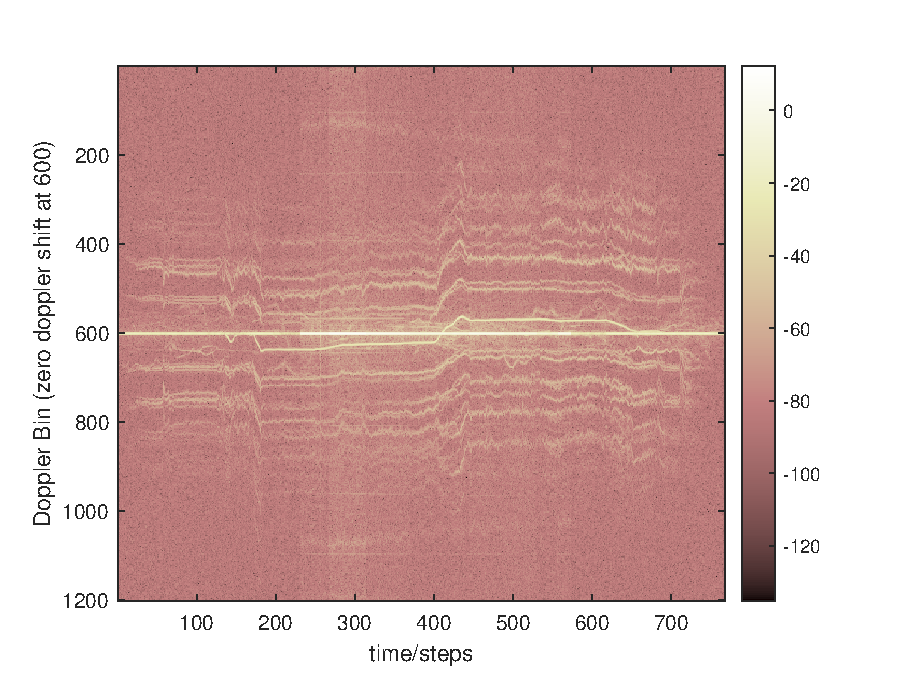
\includegraphics[scale=0.5]{Image/figure2a.eps}
    \end{minipage}
}
\subfigure[bird spectrum in the Gamekeeper dataset]
{
 	\begin{minipage}[b]{\linewidth}
        \centering
        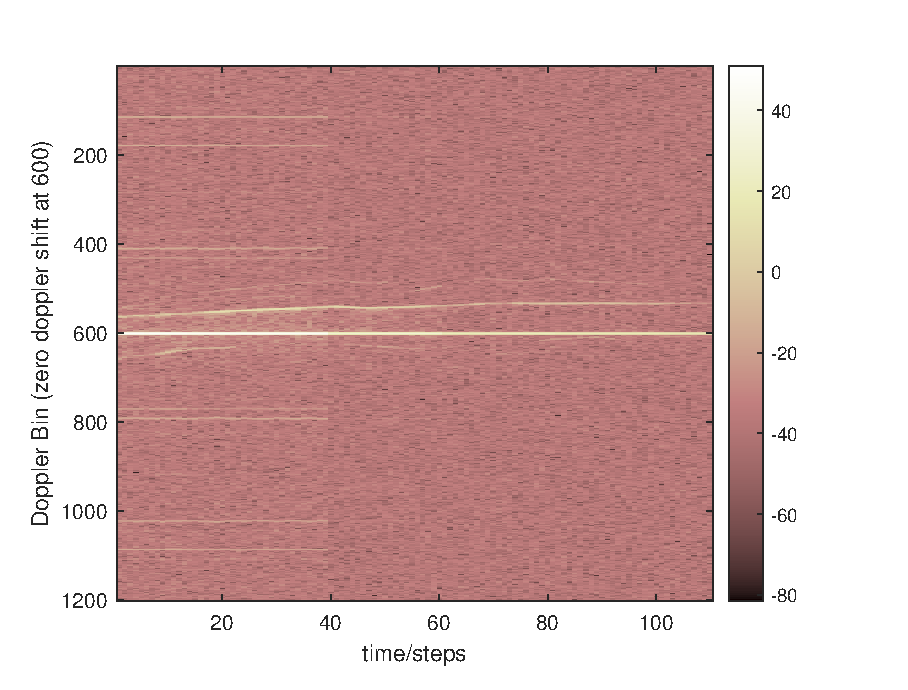
\includegraphics[scale=0.5]{Image/figure2b.eps}
    \end{minipage}
}
\caption{Example Spectrogram of Bird and Drone of Gamekeeper Dataset}
\end{figure}
Figure 2 tells clearly the difference between a bird spectrogram without the u-Doppler effect and a drone spectrogram with HERM lines in the dataset. Notice that these examples have a Doppler range of 1200Hz.

Notice that the time length for the drone spectrogram is 800 time steps and 110 time steps for the bird spectrogram. The PCA algorithm requires a uniform length for each sample, therefore the next step of the script is trimming these spectrograms. The original target spectrogram was sliced into pieces with identical lengths.
The output of the 'Gen\_Dataset.m' script is another mat file with two variables: 'label' and 'fftfrac'. The 'label' is simply a string which indicates the type of data and the 'fftfrac' is a spectrogram corresponding to the label with size of 'Doppler width(300, 600, 1200)' $\times$ '20 time steps'.
The dataset with 3006 samples is generated. A Python module 'scipy.io' is installed and the 'loadmat' function can be used to read the mat file and convert the 'fftfrac' into a numpy array. The specific code can be seen in the 'dataset.py' in the appendix.

The 'train\_test\_split' function from the 'sklearn.model\_selection' package is used to split the 3006 samples into test set and training set. The ratio used in this project is 80\% of the training set, therefore a training set of 2404 spectrograms and a test set of 602 spectrograms is generated.
\section{PCA Algorithms and Implement}
\subsection{Conventional PCA Implementation}
PCA is originally brought up my Karl Pearson in 1901 and is always a important technique when facing large data.
In this project, conventional PCA means original way of selecting the principal components of high dimensional data by maximize the variance of projected data.
The word 'conventional' is used to distinguish this method with its extension algorithms in the next sections of the project.

All PCA algorithms have the same basic idea and can be deduced in two ways: 1. The subspace has the 'maximize re-factorize', which means that the distance from original samples to the new hyperplane of the subspace should be the closest; 2. The subspace has the 'maximize separable', which means the projected data have maximum of variance.

We deduced the conventional PCA via 'maximize re-factorize':\cite{23}
Assume the training set of our data is: $\boldsymbol{X_i}: i = \{1,2,\cdots,n\}$, where $n$ is the number of data in the test set. The data has the dimension of $\boldsymbol{X} \in \mathcal{R}^{d\times n}$ where $d$ is the dimension of original data. Each column of the $\boldsymbol{X}$ represent a reshaped 1-D spectrogram.
The projection matrix of PCA is $\boldsymbol{W} =\{\boldsymbol w_1,\boldsymbol w_2\,\cdots,\boldsymbol w_d’\}$, where $d'$ is the dimension of the subspace. The projection matrix has a dimension of $\boldsymbol{W} \in \mathcal{R}^{d\times d'}$
Projected data is $\boldsymbol{Z}$,where $\boldsymbol{Z} = \boldsymbol{W}^T\cdot \boldsymbol{X}$. 
In this case, the data point in original high dimension $\boldsymbol{x}_i$ has a projected point $\boldsymbol{z}_i=\left(z_{i 1} ; z_{i 2} ; \ldots ; z_{i d^{\prime}}\right)$, where $\boldsymbol z _{ij} = w_j^T x_i$ is the $j$th dimension coordinate of the sample point in the subspace.
Therefore, the reconstructed $\hat\boldsymbol{X}$ can be expressed by: $\hat{\boldsymbol{x}}_i=\sum_{j=1}^{d^{\prime}} z_{i j} \boldsymbol{w}_j$, and then we set the objective function of conventional PCA as $\mathcal{J}_{\mathrm{obj}}$.
The distance between reconstructed data points to the original data point is:
\begin{equation}
\centering
\begin{split}
\begin{aligned}
\sum_{i=1}^m\left\|\sum_{j=1}^{d^{\prime}} z_{i j} \boldsymbol{w}_j-\boldsymbol{x}_i\right\|_2 & =\sum_{i=1}^m\left\|\mathbf{W} \boldsymbol{z}_i-\boldsymbol{x}_i\right\|_2^2 \\
& =\sum_{i=1}^m\left(\mathbf{W} \boldsymbol{z}_i-\boldsymbol{x}_i\right)^{\mathrm{T}}\left(\mathbf{W} \boldsymbol{z}_i-\boldsymbol{x}_i\right) \\
& =-\sum_{i=1}^m \boldsymbol{z}_i^{\mathrm{T}} \boldsymbol{z}_i+\text { const } \\
& =-\sum_{i=1}^m \operatorname{tr}\left(\boldsymbol{z}_i \boldsymbol{z}_i^{\mathrm{T}}\right)+\text { const } \\
& \propto -\operatorname{tr}\left(\mathbf{W}^{\mathrm{T}}\left(\boldsymbol{X} \boldsymbol{X}^{\mathrm{T}}\right) \mathbf{W}\right)\\
\end{aligned}
\end{split}
\label{eq:mi}
\end{equation}
where $\mathrm{const}$ is non-irrelevant constant value and $\mathrm{tr}$ represents the trace of matrix. According to the basic idea of PCA, minimum value of the distance in equation(1) needs to be found, hence the objective function is:
\begin{equation}
\centering
\begin{split}
\begin{aligned}
\begin{aligned}
\mathcal{J}_{\mathrm{obj}}=& \max _{\mathbf{W}}\operatorname{tr}\left(\mathbf{W}^{\mathrm{T}} \mathbf{X} \mathbf{X}^{\mathrm{T}} \mathbf{W}\right) \\
& \text { s.t. } \mathbf{W}^{\mathrm{T}} \mathbf{W}=\mathbf{I} 
\end{aligned}
\end{aligned}
\end{split}
\label{eq:mi}
\end{equation}
Problem (2) is a constrained optimization can be solved by the Lagrangian method. The Lagrangian function of the problem is:
\begin{equation}
\centering
\begin{split}
\begin{aligned}
L(\mathbf{W}, \Theta) & =\operatorname{tr}\left(\mathbf{W}^{\mathrm{T}} \mathbf{X} \mathbf{X}^{\mathrm{T}} \mathbf{W}\right)-\left\langle\Theta, \mathbf{W}^{\mathrm{T}} \mathbf{W}-\mathbf{I}\right\rangle \\
& =\operatorname{tr}\left(\mathbf{W}^{\mathrm{T}} \mathbf{X} \mathbf{X}^{\mathrm{T}} \mathbf{W}\right)-\operatorname{tr}\left(\Theta^{\mathrm{T}}\left(\mathbf{W}^{\mathrm{T}} \mathbf{W}-\mathbf{I}\right)\right)
\end{aligned}
\end{split}
\label{eq:mi}
\end{equation}
Where $\Theta \in \mathbb{R}^{d^{\prime} \times d^{\prime}}$ is the Lagrangian multiplier matrix and the elements of which are the unknown Lagrangian multiplier. Consider the constrain of object function $\boldsymbol{W}^T\boldsymbol{W}=\boldsymbol{I}$, the Lagrangian matrix should be a diagonal matrix which can be written as:
\begin{equation}
\centering
\begin{split}
\Lambda=\operatorname{diag}\left(\lambda_1, \lambda_2, \ldots, \lambda_{d^{\prime}}\right) \in \mathbb{R}^{d^{\prime} \times d^{\prime}}
\end{split}
\label{eq:mi}
\end{equation}
where the $\lambda$ is the eigenvalue of the covariance matrix of data. Substitute the equation(4) into (3), we have:
\begin{equation}
\centering
\begin{split}
L(\mathbf{W}, \Lambda)=-\operatorname{tr}\left(\mathbf{W}^{\mathrm{T}} \mathbf{X} \mathbf{X}^{\mathrm{T}} \mathbf{W}\right)+\operatorname{tr}\left(\Lambda^{\mathrm{T}}\left(\mathbf{W}^{\mathrm{T}} \mathbf{W}-\mathbf{I}\right)\right)
\end{split}
\label{eq:mi}
\end{equation}
An optimal(maximum) value of the trace can be found when the derivative of the Lagrangian function against to $\theta$ is zero, let $\partial L(\mathbf{W}, \Lambda)/\partial \mathbf{W}=\mathbf{0}$, and thus we have:
\begin{equation}
\centering
\begin{split}
\mathbf{X X}^{\mathrm{T}} \boldsymbol{w}_i=\lambda_i \boldsymbol{w}_i, \quad i=1,2, \ldots, d^{\prime}
\end{split}
\label{eq:mi}
\end{equation}
Substitute equation(6) into the objective function(2) thus we have:
\begin{equation}
\centering
\begin{split}
\mathcal{J}_{\mathrm{obj}}= \mathrm{argmax} \sum_{i=1}^{d^{\prime}} \lambda_i
\end{split}
\label{eq:mi}
\end{equation}
Therefore, the projection matrix of optimal convention PCA can be derived by combining the largest $d'$ eigenvalues of the covariance matrix $\boldsymbol{X}^T\boldsymbol{X}$.

When implementing the conventional PCA algorithm, the steps are followed:
1. Centralized test set and training set by 'StandardScaler' function from the 'sklearn preprocessing' package; 2. Calculate the covariance matrix of the test set and perform singular value decomposition(SVD) on it to calculate the eigenvalues, and then generate the eigen matrix. The Python class 'PCA' from 'sklearn.decomposition' package can be used here. The class 'PCA' has two methods that are important in the project, the 'PCA.fit' method can calculate the projection matrix of a certain test set and the 'PCA.transform' method can project the original data on the subspace; 3. Project the data onto the subspace;
Low dimension data by conventional PCA is so far produced.

The test is repeated with changing $d'$ varies from 5 to 60. The relation of classification accuracy with the dimension of subspace should be found out. The whole test is conducted on 3 groups of different Doppler shift width datasets. The specific code of conventional PCA can be found in the appendix.
\subsection{2D-PCA Implementation}
In the previous section, a conventional PCA is adopted, where each spectrogram is reshaped to 1-D and is considered as a column in $\boldsymbol{X}$. Reshaping data matrices to 1-D vectors may cause some issues on losing the spatial information.
2DPCA is developed by \cite{24} for the application of facial recognition. In their work, conventional 1-D PCA do not work well with extracting the spatial feature of human face images such as human expressions. It is proved to be an effective way of using 2DPCA on the human face dataset.
2DPCA takes into account the spatial arrangement of pixels in an image or the structure of a matrix. This means that it considers how nearby pixels interact and captures spatial patterns, edges, textures, and other local features. However, it's important to mention that 2DPCA is not always the more optimal solution than traditional PCA. Its advantages become prominent in scenarios where the spatial arrangement of data matters, such as image analysis on facial features. 

In this section, the performance impact of 2DPCA on our Gamekeeper dataset is investigated.
In 2DPCA, rather than proceeding original data matrix of $\boldsymbol{X} \in \mathcal{R}^{d\times n}$, the $i$th spectrogram in the dataset $\boldsymbol{X}_i$ is directly projected by the projection matrix $\boldsymbol{W}$. 
Let the spectrogram has the dimension of: $\boldsymbol{X}_i \in \mathcal{R}^{h\time w}$, where the $h$ and $w$ is the height and width of each spectrogram(image).
Similar to the deduction from previous section, the object function of 2DPCA can be written as:
\begin{equation}
\centering
\begin{split}
J(\mathbf{W})=\operatorname{tr}\left(\mathbf{S}_x\right)
\end{split}
\label{eq:mi}
\end{equation}
Where the $S_{(x)}$ is the covariance matrix of the projected low dimensional matrix.
Considering the relationship of projection, the covariance matrix of projected data can be expressed as:
\begin{equation}
\centering
\begin{split}
\begin{aligned}
\mathbf{S}_x & =E(\mathbf{Z}-E \mathbf{Z})(\mathbf{Z}-E \mathbf{Z})^T \\
& =E[\mathbf{W^T X}-E(\mathbf{W^T X})][\mathbf{W^T X}-E(\mathbf{W^T X})]^T \\
& =E[(\mathbf{W}-E \mathbf{W}) \mathbf{X}][(\mathbf{W}-E \mathbf{W}) \mathbf{X}]^T
\end{aligned}
\end{split}
\label{eq:mi}
\end{equation}
Where $E$ represent the centralization of data and $Z,W$ is the projected and projection matrix.
Combining the equation (9) with objective function (8), we have:
\begin{equation}
\centering
\begin{split}
\begin{aligned}
\mathcal{J}(\mathbf{W}) & = \operatorname{tr}\left(\mathbf{S}_x\right) \\
& = \mathbf{W}^T\left[E(\mathbf{X}-E \mathbf{X})^T(\mathbf{X}-E \mathbf{X})\right] \mathbf{W}\\
& = \mathbf{W}^T \frac{1}{n} \sum_{j=1}^n\left(\mathbf{X}_j-\overline{\mathbf{X}}\right)^T\left(\mathbf{X}_j-\overline{\mathbf{X}}\right) \mathbf{W}
\end{aligned}
\end{split}
\label{eq:mi}
\end{equation}
Consider the $\frac{1}{n} \sum_{j=1}^n\left(\mathbf{X}_j-\overline{\mathbf{X}}\right)^T\left(\mathbf{X}_j-\overline{\mathbf{X}}\right)$ as the image scatter matrix $\boldsymbol{G}$. It's straightforward that the $\mathcal{J}$ has a maximum value when the $\boldsymbol{W}$ is the listing of largest eigenvalue of $\boldsymbol{G}$.
In a word, the 2DPCA substitute the covariance matrix of original data in conventional PCA to the covariance matrix of the average value of all spectrograms.

In the implementation of 2DPCA, no ready-made algorithm package is used and the code is designed based on the deduction from previous content.
The pseudo-code of 2DPCA for this project is shown in algorithm 1:

\begin{algorithm}[H]
 \KwData{Spectrogram Dataset, dimension of subspace $d'$ }
 \KwResult{Projected matrix for 2DPCA $\boldsymbol{Z}$}
 initialization(Do not centralized the data)\;
 \While{i<n}{
  $G = \frac{1}{n} \sum_{j=1}^n\left(\mathbf{X}_j-\overline{\mathbf{X}}\right)^T\left(\mathbf{X}_j-\overline{\mathbf{X}}\right)$\;
  Eigenvalue Decomposition $G$\;
  Get largest $d'$ Eigenvalue;
  $\boldsymbol{W} = (w_1,w_2,\cdots,w_{d'})$\;
  $\boldsymbol{Z} = \boldsymbol{W}^T \boldsymbol{X}$\;
  i++\;
 }
 \caption{2D-PCA}
\end{algorithm}
The eigenvalue decomposition step can be achieved by the 'linalg.eig' method in the numpy package. The rest of the steps in the pseudo-code are relativity simple.
The test on 2DPCA repeated from $d' = 5$ to $d' =60$. Each projected matrix is used to train an SVM classifier. The accuracy is then calculated to evaluate the performance of 2D-PCA.
\subsection{PCA with L1-Norm Implementation}
L1-Norm Based PCA is first brought up in \cite{25}. 
Generally speaking, the implementation of L1 distance in the optimization of object function in machine learning can increase the robustness of the model. There are a few reasons for the robustness: firstly, the L2 norm directly uses the Euclidean Distance, which is the square value of data points' deviations from the central point. This means that the impact of large positive and negative deviations, which is considered abnormal samples in the dataset, are amplified. This lack of sensitivity to outliers is why the L2 norm is not considered robust in the presence of extreme values. However, the L1 norm treated the distance equally, which is more robust to abnormal points. 
Secondly, when minimizing the L1 norm, the solutions tend to be sparse, which means that many components of the solution vector are exactly zero. Outliers can have a reduced effect on the solution because their influence on the objective function is limited by the absolute value penalty.
The outlier in this project could mean the data points that significantly deviate from the overall pattern or distribution of data in an image or a dataset. The reason of the outlier could be noise, mislabelled data or a unique target.
Moreover, the L1-norm in PCA brings sparse to the subspace, more zeros in the feature space and could make the main components contain more valuable information than conventional PCA.

The L1-Norm PCA problem is similar to the conventional L2-Norm PCA. Only the distance is measured in Manhattan distance rather than Euclidean distance. The distance is expressed by:
\begin{equation}
\sum_{i=1}^m\left\|\sum_{j=1}^{d^{\prime}} z_{i j} \boldsymbol{w}_j-\boldsymbol{x}_i\right\|_1=\sum_{i=1}^m\left\|\mathbf{W} \boldsymbol{z}_i-\boldsymbol{x}_i\right\|_1
\end{equation}
Similar to the proof in section 3.1, the object function of L1-PCA can be deduced by maximize the dispersion of reconstruct images. 
\begin{equation}
\begin{aligned}
& \mathcal{J}=\underset{W}{\arg \max }\left\|\bold W^T \bold X\right\|_1=\underset{\bold W}{\arg \max } \sum_{i=1}^n \sum_{k=1}^{d'}\left|\sum_{j=1}^d w_{j k} x_{j i}\right|_1 \\
& \text { s.t.} \bold W^T \bold W=\bold{I_m} .
\end{aligned}
\end{equation}
Notice that in the conventional PCA and 2DPCA, the optimal value of projection matrix $W$ is not independent against $d'$. In other word, in the conventional scenario, the subspace with lower dimension is always the subset of the larger ones, because the rank of eigenvalue is fixed. However, in L1PCA, the optimal $i$th  projection vector $w_i$ will vary as $d'$ changes.

Therefore it is not easy to find a global maximum value of the objective function. In \cite{25}, a sub-optimal solution is given based on the similarity. The optimal projection matrix when $d'>1$ can be approximate by the optimal projection matrix when $d'=1$. A greedy search algorithm in \cite{25} is proposed based on the fixed point iteration method. More efficient algorithm has been developed in \cite{26}. The \cite{26} provides a non-greedy search algorithm to solve the problem (12) with iterative alternating optimization and proved to have a better accuracy on classifier.

The method used in this project is a optimal algorithm using iteration via bit-flapping based on the work of \cite{27}.
The problem of L1PCA showed in equation (12) can be expressed by: \cite{28}
\begin{equation}
\begin{aligned}
\mathbf{B}_{\mathrm{opt}}=\underset{\mathbf{B} \in\{ \pm 1\}^{N \times K}}{\operatorname{argmax}}\|\mathbf{X B}\|_*,
\end{aligned}
\end{equation}
and
\begin{equation}
\mathbf{W}=U\left(\mathbf{X B}_{\mathrm{opt}}\right)
\end{equation}
Where $U(\bold X)$ represent the $\boldsymbol{U}$ matrix in the SVD of $\boldsymbol{X} = \boldsymbol{U} \boldsymbol{\Lambda} \boldsymbol{V}$. $\mathbf{B} \in\{ \pm 1\}^{N \times K}$ refers to a binary matrix where all elements is either -1 or 1. \cite{27} provide a proof that the equation(13) can be written in a more simple form of:
\begin{equation}
\mathbf{B}_{\text {opt }}=\underset{\mathbf{B} \in\{ \pm 1\}^{N \times K}}{\operatorname{argmax}}\|\mathbf{Y B}\|_*,
\end{equation}
where $\bold Y = \Lambda \bold V$ has a dimension less than $\boldsymbol{X}$ and will same some computation. Then the optimal value of projection matrix can be calculated by iteration of finding a optimal value of $\boldsymbol{B}$.
Before the iteration, a array of $L$ with the length of $nd'$ indicates all the element that haven't been flipped.
In each iteration, the algorithm go through all elements of binary matrix $\boldsymbol{B}$ by flipping them. Changing in L1 norm will be measured after each flipping and the maximum value of increasing will be record. The optimal flipping element corresponding to the maximum L1 norm increase will be update to next iteration. 
The principal idea of L1 norm maximization via bit flipping is shown in the pseudo code of algorithm 2.
\begin{algorithm}[H]
 \KwData{Spectrogram Dataset$\boldsymbol{X}$ dimension of subspace $d'$ }
 \KwResult{Projection matrix for L1PCA $\boldsymbol{W}$}
    initialization(Centralized the data)\;
    $\left(\mathbf{U}, \mathbf{\Lambda}_{d \times d}, \mathbf{V}\right) \leftarrow \operatorname{svd}(\mathbf{X})$\;
    $\mathbf{Y} \leftarrow \mathbf{\Sigma} \mathbf{V}^{\top}, \mathbf{v} \leftarrow[\mathbf{V}]_{:, 1}$\;
    $\text{Initialize} B, \mathbf{B}=\operatorname{sgn}\left(\mathbf{v} \mathbf{1}_K^{\top}\right)$\;
    \While{not convergence, i<nd'}{
        \While{j<nd'}{
        Bit Flapping\;
        j++\;
        }
    i++\;
     }
     $\left(\hat{\mathbf{U}}_{d \times d'}, \hat{\boldsymbol{\Sigma}}_{d' \times d'}, \hat{\mathbf{V}}_{d' \times d'}\right) \leftarrow \operatorname{svd}\left(\mathbf{X B}_{\mathrm{bf}}\right)$\;
     $\mathbf{W} \leftarrow \hat{\mathbf{U}} \hat{\mathbf{V}}^{\top}$
 \caption{L1-PCA}
\end{algorithm}
Convergence proof and computation cost are further discussed in \cite{27}. 
The source code of L1PCA is shown in the appendix. Algorithm 2 implements modification on a function 'l1pca\_sbfk', which is from an open-source program. 
The test on L1PCA is repeated from 5 to 60 main component extractions. The trial is performed with the spectrogram dataset of 600Hz Doppler range due to the limit of hardware(The 1200Hz spectrograms are too large for the RAM). The performance of L1PCA can be analyzed to tell the differences between these algorithms.
SVM classifier is trained by the space data with the same kernel function as the previous section.

\subsection{Testbed of SVM Classifier}
The main goal of the SVM algorithm is to find a hyperplane that can correctly separate data points of different classes with maximum margin.
In our binary classification problem of birds and drones, the SVM produce a boundary between two clusters of data point in the subspace after PCA.
The SVM Classifier testbed is implement by 'sklearn.svm' package.
A typical SVM classifier can be set with the hyper-parameters shows below:
\lstset{language = python}
\begin{lstlisting}
"C": loguniform(1e3, 1e5),
"gamma": loguniform(1e-4, 1e-1),
kernel: "rbf" 
class_weight: "balanced"
\end{lstlisting}
where the "C" controls the regularization strength, and "gamma" is a parameter for the radial basis function (RBF) kernel. 
The Support Vector Classification (SVC) class is instanced with a radial basis function (RBF) kernel and "balanced" class weights. 
The RBF kernel is often used for SVMs when dealing with non-linearly separable data, which could be suitable for image classification, and the "balanced" class weights help address class imbalance issues in the training data.

It needs to be noted that the selection of parameters in SVM is not intended to create an "optimal" classifier that can offer greater accuracy. The SVM model is just a shallow machine learning model when compared to a deep learning algorithm, and hence is only used as a testbed for the PCA algorithms. The SVM model can be trained quickly and efficiently. 
What needs to be assured is that the parameters remain the same for each trial of PCA.
\section{Classification Result and Analysis}
\subsection{Principals of Trials}
The performance of the PCA is measured by these several metrics: accuracy, precision, recall, F1-score and confusion matrix. 
The macro accuracy is the simple average of the accuracy calculated for each class individually. It treats all classes equally and doesn't take class imbalances into account. It's calculated by summing up the accuracies for each class and then dividing by the total number of classes; 
The precision of each class measures the ratio of correctly predicted positive data points to the total data points predicted as positive;
Recall is the sensitivity and the true positive rate, it's the ratio of number of correctly prediction to the total actual positive predictions.
The calculation of the precision and recall is shown in equation (16).
\begin{equation}
\begin{aligned}
\text { Precision } & =\frac{\text{Correctly Predict Positive}}{\text{All Positive}} \\
\text { Recall } & =\frac{\text{Correctly Predict Positive}}{\text{All Correct Prediction}}
\end{aligned}
\end{equation}
The F1 score is a metric that combines both precision and recall into a single value, providing a balanced view of a model's performance in a binary or multi-class classification scenario. F1 score is particularly useful when the precision and recall are both need to be considered. The calculation of the F1 score is shown in the equation (17).
\begin{equation}
F 1=\frac{2 \times \text { Precision } \times \text { Recall }}{\text { Precision }+ \text { Recall }}
\end{equation}
Confusion matrix of a model is a more intuitive way of demonstrating the performance of the algorithm. A typical confusion matrix is a square matrix with rows and columns corresponding to the classes in your dataset. The main components of each cell in the confusion matrix are true positive(Correctly predicted in the class), true negative(correctly predicted outside the class), false positive(incorrectly predicted in the class) and false negative(incorrectly predicted out the class).
Time cost as another metric is considered as well. The time for dimension reduction and training an SVM classifier is measured. Ideally, PCA dimension reduction will save the computation of SVM.
\begin{table*}[!b]
\renewcommand{\arraystretch}{1.5}
\caption{Metrics Measured by 12 Trials, PCA reconstruction with 60 main components}
\begin{center}
\begin{tabular}{|c|c|c|c|c|c|c|c|c|c|}

\hline
\textbf{Metric}& \textbf{Time for PCA}& \textbf{Time for SVM}& \textbf{Precision} & \textbf{Precision} & \textbf{Recall} & \textbf{Recall} & \textbf{F1 score} & \textbf{F1 score} & \textbf{Avg Accuracy}\\

\textbf{Class of Target:}& (s) & (s) & \textbf{\textit{birds}} & \textbf{\textit{drones}} & \textbf{\textit{birds}} & \textbf{\textit{drones}} & \textbf{\textit{birds}} & \textbf{\textit{drones}} & & 
\hline
\cline{2-12} 

\hline
\textbf{\textit{without-PCA300}} & N/A & 521.71 & 0.73 & 0.83 & 0.77 & 0.79 & 0.75 & 0.81 & 0.78  \\
\hline
\textbf{\textit{without-PCA600}} & N/A & 1209.85 & 0.90 & 0.87 & 0.80 & 0.93 & 0.85 & 0.90 & 0.88  \\
\hline
\textbf{\textit{without-PCA1200}} & N/A & 2185.63 & 0.83 & 0.92 & 0.89 & 0.87 & 0.86 & 0.89 & 0.88  \\
\hline
\textbf{\textit{conv-PCA300}} & 0.54 & 22.54 & 0.57 & 0.89 & 0.91 & 0.52 & 0.70 & 0.65 & 0.68  \\
\hline
\textbf{\textit{conv-PCA600}} & 0.90 & 11.83 & 0.76 & 0.95 & 0.94 & 0.79 & 0.84 & 0.86 & 0.85  \\
\hline
\textbf{\textit{conv-PCA1200}} & 1.74 & 15.87 & 0.76 & 0.94 & 0.93 & 0.79 & 0.84 & 0.86 & 0.85  \\
\hline
\textbf{\textit{2D-PCA300}} & (0.94) & 164.40 & 0.66 & 0.84 & 0.82 & 0.69 & 0.73 & 0.76 & 0.75  \\
\hline
\textbf{\textit{2D-PCA600}} & (1.40) & 153.90 & 0.67 & 0.81 & 0.75 & 0.73 & 0.71 & 0.77 & 0.74  \\
\hline
\textbf{\textit{2D-PCA1200}} & (3.44) & 145.84 & 0.66 & 0.84 & 0.82 & 0.70 & 0.73 & 0.76 & 0.75 \\
\hline
% \textbf{\textit{L1-PCA300}} & 24174 & 189 & 3 & 6 & 274 & 356 & 96.69 & 1 & 1 \% \\
% \hline
\textbf{\textit{L1-PCA600}} & 19352 & 24.02 & 0.88 & 0.91 & 0.87 & 0.91 & 0.88 & 0.91 & 0.90 \\
\hline
% \textbf{\textit{L1-PCA1200}} & 24174 & 189 & 3 & 6 & 274 & 356 & 96.69 & 1 & 1 \% \\
% \hline
\end{tabular}
\label{tab7}
\end{center}
\end{table*}

In the project, 10 instantiations(trails) of the SVM model are trained and three PCA preprocessing algorithms are used on them:
\begin{itemize}
    \item without-PCA300: The comparison group of the SVM model trained by original data without PCA. Original data are spectrograms which have a Doppler width of 300Hz.
    \item without-PCA600: The comparison group of the SVM model trained by original data without PCA. Original data are spectrograms which have a Doppler width of 600Hz.
    \item without-PCA1200: The comparison group of the SVM model trained by original data without PCA. Original data are spectrograms which have a Doppler width of 1200Hz.
    \item conv-PCA300: The test group of the SVM model trained by original data with conventional PCA. Original data are spectrograms which have a Doppler width of 300Hz. PCA use 5 to 60 components. 
    \item conv-PCA600: The test group of the SVM model trained by original data with conventional PCA. Original data are spectrograms which have a Doppler width of 600Hz. PCA use 5 to 60 components.
    \item conv-PCA1200: The test group of the SVM model trained by original data with conventional PCA. Original data are spectrograms which have a Doppler width of 1200Hz. PCA use 5 to 60 components.
    \item 2D-PCA300: The second test group of the SVM model trained by original data with 2DPCA. Original data are spectrograms which have a Doppler width of 300Hz. PCA use 5 to 60 components.
    \item 2D-PCA600: The second test group of the SVM model trained by original data with 2DPCA. Original data are spectrograms which have a Doppler width of 600Hz. PCA use 5 to 60 components.
    \item 2D-PCA1200: The second group of the SVM model trained by original data with 2DPCA. Original data are spectrograms which have a Doppler width of 1200Hz. PCA use 5 to 60 components.
    % \item L1-PCA300: The third group of the SVM model trained by original data with L1PCA. Original data are spectrograms which have a Doppler width of 600Hz. PCA use 5 to 60 components.
    \item L1-PCA600: The third group of the SVM model trained by original data with L1PCA. Original data are spectrograms which have a Doppler width of 600Hz. PCA use 5 to 60 components.
    % \item L1-PCA1200: The third group of the SVM model trained by original data with L1PCA. Original data are spectrograms which have a Doppler width of 600Hz. PCA use 5 to 60 components.
\end{itemize}
\subsection{Demonstration and Analysis of Result}
Table 1 shows metrics measured in the trials of this project. The conventional PCA, 2DPCA and L1PCA data are gathered from the trial where the 60 largest principal components are used as subspace. 
The trial is conducted two times. For the first time, CPU computation is implemented with traditional Numpy and Scipy packages. The second time, GPU is involved by cupy packages in solving the matrices during 2DPCA and L1PCA.
In Table 1, brackets in the column of time metric refer to time consumption when the projection matrices are solved by GPU.
The metrics are tested with a hardware platform of "Intel 6-cores i7" with a main frequency at 2.6GHZ plus "Nvidia GTX 1650" with a CUDA computation ability of 7.5.
\subsubsection{Accuracy Analysis}
Comparing the metrics of the SVM classifier without PCA preprocessing, it shows a trend of increasing macro accuracy when the width of Doppler frequency increases. 
The metric of average accuracies shows that, for an SVM classifier, most of the features that can distinguish the birds and drones lie within the u-Doppler range of -300Hz to 300Hz, since the accuracies are the same for the last two trials.
The confusion matrix of SVM without PCA of 1200Hz range is shown in Figure 3.
\begin{figure}[h]
\centering\includegraphics[scale = 0.5]{Image/without_PCA1201binCFM.png}
\caption{Confusion Matrix for Trial 'without-PCA1200'}
\end{figure}
The figure shows that the classifier has a higher chance of predicting a bird target as a drone.
The classification accuracy of SVM towards the original data may be a mediocre result and less competitive to advanced classifiers. However, it is only a benchmark of algorithm performance. 

As for the conventional PCA algorithm. The metrics show that the performance of SVM with PCA dimension reduction is close to the SVM trained by the original data, with only a few percent drop in the average accuracy.
However the trial with 300Hz wide u-Doppler spectrograms is different, the performance of it is extremely poor. The reason for this may be the effective principal components lie in the 150 to 300Hz Doppler shift. 
Figure 4 is the confusion matrix of the trial 'conv-PCA1200'.
\begin{figure}[h]
\centering\includegraphics[scale = 0.5]{Image/ConvPCA_with1201binCFM60.png}
\caption{Confusion Matrix for Trial 'conv-PCA1200'}
\end{figure}
Generally speaking, the conventional PCA has a better Recall on bird classification than without PCA, yet the F1 scores and macro accuracy are nearly the same. Moreover, the conventional PCA preprocessing in this case will make the SVM more sensitive to the 'edge-spectrogram' data(part of a spectrogram with Doppler shifting larger than 150Hz). Conventional PCA with the Gamekeeper dataset will bring misclassified drones as birds, as shown in Figure 4.

The performance of 2DPCA is not ideal enough compared to its performance on other datasets\cite{24}. 
The accuracy of SVM trained with 2DPCA preprocessing is 10\% lower than conventional PCA implementation. 
The F1 score of each class is poor in the 2DPCA as well. 
Now from the result of this project, we can say that the 2DPCA is not suitable for preprocessing the Gamekeeper dataset, however, the reason for this could be varied.
One possible reason could be that the 2DPCA is focusing on the two-dimensional feature of the images however, the spectrograms of radar targets contain more important features in only one direction. For instance, 1-D PCA treats the spectrogram as an array and important features for classification such as HERM lines are parallel to the time-step axis. Therefore using 2DPCA on the radar dataset might just not correspond to the nature of the dataset.
Another possible reason is different preprocessing techniques have varying sensitivities to noise and outliers. If the radar data contains noise or outlier points that are not handled well by 2DPCA, it could negatively impact its performance. 
In a word, the effectiveness of preprocessing techniques can be highly dependent on the characteristics of the data. The structure, noise level, distribution, and other features of spectrogram data might be better suited for conventional PCA rather than 2DPCA.
The reason for this result could be complicated and sophisticated, yet a valuable outcome is concluded, which is, that the 2DPCA is not suitable in this scenario and may not be suitable for any model that is trained with the Gamekeeper dataset.
Figure 5 shows the confusion matrix from trial '2D-PCA1200'. 
\begin{figure}[h]
\centering\includegraphics[scale = 0.5]{Image/2DPCA_with1201binCFM60.png}
\caption{Confusion Matrix for Trial '2D-PCA1200'}
\end{figure}
It can be seen from it that the precision is poor.
Moreover, the 2DPCA algorithm has performance nearly the same when the spectrograms in the dataset have different widths, which indicates that the 2DPCA will make SVM less sensitive to the 'edge-spectrogram'. 

As for L1PCA performance. Comparing the 'L1-PCA600Hz' trial with other trials with a width of 600Hz shows that the L1-PCA has the best performance among the three algorithms. 
Not only does the L1-PCA have the highest F1 scores and macro accuracy, but it also shows the balance of precision and recall. The precision and recall of the two classes are both nearly 0.9. Figure 6 shows the confusion matrix of this trial.
\begin{figure}[h]
\centering\includegraphics[scale = 0.5]{Image/L1PCA_with601binCFM60.png}
\caption{Confusion Matrix for Trial 'L1-PCA600'}
\end{figure}
The effectiveness of the L1-PCA preprocessing could be because noise and outlier exist in the original dataset, and the robustness of L1-PCA boost the performance of the model.
Moreover, L1-PCA encourages sparse solutions, meaning that some components of the resulting representation can be exactly zero. This property can be advantageous when dealing with high-dimensional data where not all features are relevant. Sparse solutions might lead to better feature selection, making the data more informative for classification.
Overall, the success of L1-PCA could be attributed to a combination of its ability to handle outliers, its sparsity-inducing nature, and its capacity to extract informative features from the radar spectrogram data.

The figure 7 shows the accuracy changing against the number of main components in the algorithm.
\begin{figure*}[!t]
\centering
\subfigure[Conventional PCA]
{
    \begin{minipage}[b]{0.31\linewidth}
        \centering
        \includegraphics[scale=0.4]{Image/ConvPCA_with601bin.png}
    \end{minipage}
}
\subfigure[2D-PCA]
{
 	\begin{minipage}[b]{0.31\linewidth}
        \centering
        \includegraphics[scale=0.4]{Image/2DPCA_with601bin.png}
    \end{minipage}
}
\subfigure[L1-PCA]
{
 	\begin{minipage}[b]{0.31\linewidth}
        \centering
        \includegraphics[scale=0.4]{Image/L1PCA_with601bin.png}
    \end{minipage}
}
\caption{Accuracy vs. Number of Components of difference PCA algorithm preprocessing}
\end{figure*}
In figure 7, it shows that the performance of L1-PCA is better than other algorithms whatever number of $d'$ is chosen.
The conventional PCA shows a higher accuracy as the number of components rises, and 2D-PCA and L1-PCA show a relatively uniform value of accuracy against the number of components.
It means that in 2D-PCA and L1-PCA, the information about classification is concentrated in the first several components. As for the conventional PCA which has a larger 'slope', the rest of the components contain some of the information and adding them into the SVM will boost the performance.
Therefore the efficiency of 2D-PCA and L1-PCA is higher.
\subsubsection{Time Consumption Analysis}
Noticing that the time consumption metric in Table 1 is not a precise reflection on the computation of the algorithm, because the hardware performance is not always stable. Yet comparisons and some conclusions can still be made.
The Training time for SVM without a PCA preprocessing cost 500 to 2000 second. In the rest of the trials, this step will only cost less than 200 seconds. Especially for L1-PCA with 600Hz width, it boosts the time cost for training SVM over 10 times faster compared to no-PCA with 600Hz width.
For the conventional and 2D PCA algorithms, the cost of time is very limited. However, the L1-PCA algorithm has a heavy computation of over 19000s.

Using L1-PCA that costs 19000s to trade for 10 times faster SVM training seems to increase the computation, however, the SVM model is only a benchmark and the classifier model in the real application in radar result processing could be much more complicated than an SVM model and larger dataset. 
Comparing the L1-PCA and conventional PCA, there is a trade-off between computation and performance.
\section{Conclusion}\label{sec10}
This project compares the impact of three PCA algorithms on the performance of the classifier of the UoB Gamekeeper radar dataset. The L1-PCA algorithm is proved to be the optimal algorithm for preprocessing the spectrogram dataset due to its robustness. The Conventional and L1-PCA algorithms not only reduce the complexity of the dataset used to train machine learning models but also increase the accuracy of models.
2DPCA is not suitable for this particular spectrogram dataset when facing a classification problem of birds and drones.
PCA is well known for its anti-noise ability, and future works could explore the impact of the PCA algorithm when the dataset is corrupted by noise. More PCA algorithms are still waiting to be implemented with the Gamekeeper dataset.
\section{Acknowledgments}\label{sec11}
This paper is a report on the University of Birmingham MSc Program Final Year Project. The project was came up with and under the supervision of Dr Michail Antoniou. The author wants to express his thanks to Dr Mohammed Jahangir and Me Daniel White, who provided instruction on this work.


\newpage
\begin{thebibliography}{9}
\bibitem{1}
'Are drones really dangerous to airplanes?' - https://theconversation.com/are-drones-really-dangerous-to-airplanes-56770, accessed 15 Augst 2023

\bibitem{2}
M. Jahangir and C. Baker, "Robust Detection of Micro-UAS Drones with L-Band 3-D Holographic Radar," 2016 \textit{Sensor Signal Processing for Defence (SSPD)}, Edinburgh, UK, 2016, pp. 1-5, doi: 10.1109/SSPD.2016.7590610.

\bibitem{3}
Torvik, B., Olsen, K.E. and Griffiths, H., 2016. Classification of birds and UAVs based on radar polarimetry. \textit{IEEE geoscience and remote sensing letters}, \textbf{13(9)}, pp.1305-1309.

\bibitem{4}
Srigrarom, S., Chew, K.H., Da Lee, D.M. and Ratsamee, P., 2020, September. Drone versus bird flights: Classification by trajectories characterization. In 2020 59th \textit{Annual Conference of the Society of Instrument and Control} Engineers of Japan (SICE) (pp. 343-348). IEEE.

\bibitem{5}
Saqib, M., Khan, S.D., Sharma, N. and Blumenstein, M., 2017, August. A study on detecting drones using deep convolutional neural networks. In 2017 14th \textit{IEEE international conference on advanced video and signal based surveillance (AVSS)} (pp. 1-5). IEEE.


\bibitem{6}
Chen, V.C., 2019. \textit{The micro-Doppler effect in radar}. (pp. 105-136) Artech house.

\bibitem{7}
Klaer, P., Huang, A., Sévigny, P., Rajan, S., Pant, S., Patnaik, P. and Balaji, B., 2020. An investigation of rotary drone HERM line spectrum under manoeuvering conditions. \textit{Sensors}, 20(20), p.5940.

\bibitem{8}
Dale, H., Baker, C., Antoniou, M. and Jahangir, M., 2020, April. An initial investigation into using convolutional neural networks for classification of drones. In 2020 \textit{IEEE International Radar Conference (RADAR)} (pp. 618-623). IEEE.

\bibitem{9}
Harmanny, R.I.A., De Wit, J.J.M. and Cabic, G.P., 2014, October. Radar micro-Doppler feature extraction using the spectrogram and the cepstrogram. In \textit{2014 11th European Radar Conference} (pp. 165-168). IEEE.

\bibitem{10}
Zhang, W., Li, G. and Baker, C., 2020. Radar recognition of multiple micro‐drones based on their micro‐Doppler signatures via dictionary learning. \textit{IET Radar, Sonar & Navigation}, 14(9), pp.1310-1318.

\bibitem{11}
Hanif, A., Muaz, M., Hasan, A. and Adeel, M., 2022. Micro-Doppler based target recognition with radars: A review. \textit{IEEE Sensors Journal}, 22(4), pp.2948-2961.

\bibitem{12}
Jahangir, M., Atkinson, G.M., White, D., Griffiths, D., Ren, X., Wayman, J.P., Baker, C.J., Sadler, J.P., Reynolds, S.J. and Antoniou, M., 2022, October. Networked staring radar testbed for urban surveillance: status and preliminary results. \textit{In International Conference on Radar Systems (RADAR 2022)} (Vol. 2022, pp. 471-476). IET.

\bibitem{13}
Jahangir, M., Atkinson, G.M., Antoniou, M., Baker, C.J., Sadler, J.P. and Reynolds, S.J., 2021, June. Measurements of birds and drones with L-band staring radar. In 2021 21st International Radar Symposium (IRS) (pp. 1-10). IEEE.

\bibitem{14}
Jahangir, M., Baker, C.J. and Oswald, G.A., 2017, May. Doppler characteristics of micro-drones with L-Band multibeam staring radar. In 2017 \textit{IEEE Radar Conference (RadarConf)} (pp. 1052-1057). IEEE.

\bibitem{15}
Sim, J., Jahangir, M., Fioranelli, F., Baker, C.J. and Dale, H., 2019, September. Effective ground-truthing of supervised machine learning for drone classification. In \textit{2019 International Radar Conference (RADAR)} (pp. 1-5). IEEE.

\bibitem{16}
Jahangir, M., Ahmad, B.I. and Baker, C.J., 2020, April. Robust drone classification using two-stage decision trees and results from SESAR SAFIR trials. In \textit{2020 IEEE International Radar Conference (RADAR)} (pp. 636-641). IEEE.

\bibitem{17}
Dale, H., Jahangir, M., Baker, C.J., Antoniou, M., Harman, S. and Ahmad, B.I., 2022, March. Convolutional Neural Networks for Robust Classification of Drones. In \textit{2022 IEEE Radar Conference (RadarConf22)} (pp. 1-6). IEEE.

\bibitem{18}
Dale, H., Baker, C., Antoniou, M., Jahangir, M. and Atkinson, G., 2021, May. A comparison of convolutional neural networks for low SNR radar classification of drones. In \textit{2021 IEEE Radar Conference (RadarConf21)} (pp. 1-5). IEEE.

\bibitem{19}
Dale, H., Baker, C., Antoniou, M., Jahangir, M., Atkinson, G. and Harman, S., 2022. SNR‐dependent drone classification using convolutional neural networks. \textit{IET Radar, Sonar & Navigation}, \textbf{16}(1), pp.22-33.

\bibitem{20}
Guo, Y., Zhou, Y. and Zhang, Z., 2021. Fault diagnosis of multi-channel data by the CNN with the multilinear principal component analysis. \textit{Measurement}, 171, p.108513.

\bibitem{21}
Zhai, X., Jelfs, B., Chan, R.H. and Tin, C., 2016, August. Short latency hand movement classification based on surface EMG spectrogram with PCA. In \textit{2016 38th annual international conference of the IEEE engineering in medicine and biology society (EMBC)} (pp. 327-330). IEEE.

\bibitem{22}
Zhang, P., Yang, L., Chen, G. and Li, G., 2017, November. Classification of drones based on micro-Doppler signatures with dual-band radar sensors. In \textit{2017 Progress in Electromagnetics Research Symposium-Fall (PIERS-FALL)} (pp. 638-643). IEEE.

\bibitem{23}
Zhou, Zhi-Hua. \textit{Machine learning}. (pp. 247-263)Springer Nature, 2021.

\bibitem{24}
Yang, J., Zhang, D., Frangi, A.F. and Yang, J.Y., 2004. Two-dimensional PCA: a new approach to appearance-based face representation and recognition. \textit{IEEE transactions on pattern analysis and machine intelligence}, \textbf{26(1)}, pp.131-137.

\bibitem{25}
Kwak, N., 2008. Principal component analysis based on L1-norm maximization. \textit{IEEE transactions on pattern analysis and machine intelligence}, \textbf{30(9)}, pp.1672-1680.

\bibitem{26}
Nie, F., Huang, H., Ding, C., Luo, D. and Wang, H., 2011, July. Robust principal component analysis with non-greedy l1-norm maximization. In \textit{IJCAI proceedings-international joint conference on artificial intelligence} (Vol. 22, No. 1, p. 1433).

\bibitem{27}
Markopoulos, P.P., Kundu, S., Chamadia, S. and Pados, D.A., 2017. Efficient L1-norm principal-component analysis via bit flipping. \textit{IEEE Transactions on Signal Processing}, \textbf{65(16)}, pp.4252-4264.

\bibitem{28}
Markopoulos, P.P., Karystinos, G.N. and Pados, D.A., 2013, August. Some options for L1-subspace signal processing. In ISWCS 2013; \textit{The Tenth International Symposium on Wireless Communication Systems} (pp. 1-5). VDE.
\end{thebibliography}
\vfill\pagebreak
\section{Appendices}\label{sec14}
The project is open source on github: \newline
https://github.com/sirius0414/drone\_classification.git\newline
Only a certain amount of core source code and output logs is provided here due to page limit.
\subsection{Output Logs(Part of)}
\lstset{language = Matlab}
\begin{lstlisting}
Dataset instantiation in 1.065s
Size of train data: 2404
Size of test data: 602
-------------------------------------------------------
Read-300bin
Best estimator found by grid search:
SVC(C=70303.92448712011, class_weight='balanced', gamma=0.0016230383891044757)
time for SVM: 521.712s
              precision    recall  f1-score   support
       Drone       0.83      0.79      0.81       351
        Bird       0.73      0.77      0.75       251
    accuracy                           0.78       602
   macro avg       0.78      0.78      0.78       602
weighted avg       0.78      0.78      0.78       602
-------------------------------------------------------
Dataset instantiation in 90.303s
Size of train data: 2404
Size of test data: 602
-------------------------------------------------------
Read-600bin
Best estimator found by grid search:
SVC(C=6892.49536284177, class_weight='balanced', gamma=0.002034973644889487)
time for SVM: 1209.950s
              precision    recall  f1-score   support
       Drone       0.87      0.93      0.90       351
        Bird       0.90      0.80      0.85       251
    accuracy                           0.88       602
   macro avg       0.88      0.87      0.87       602
weighted avg       0.88      0.88      0.88       602
-------------------------------------------------------
Dataset instantiation in 47.503s
Size of train data: 2404
Size of test data: 602
-------------------------------------------------------
Read-1200bin
Best estimator found by grid search:
SVC(C=1027.600849076076, class_weight='balanced', gamma=0.0002448132690543083)
time for SVM: 2185.632s
              precision    recall  f1-score   support
       Drone       0.92      0.87      0.89       351
        Bird       0.83      0.89      0.86       251
    accuracy                           0.88       602
   macro avg       0.87      0.88      0.87       602
weighted avg       0.88      0.88      0.88       602
-------------------------------------------------------
Dataset instantiation in 35.858s
Size of train data: 2404
Size of test data: 602
Best estimator found by grid search:
SVC(C=11986.907045662787, class_weight='balanced', gamma=0.056617586035960864)
              precision    recall  f1-score   support
       Drone       0.98      0.36      0.53       351
        Bird       0.53      0.99      0.69       251
    accuracy                           0.63       602
   macro avg       0.76      0.68      0.61       602
weighted avg       0.79      0.63      0.60       602
-------------------------------------------------------
 Conv PCA with 5 components
PCA with 5 components done in 18.115s
-------------------------------------------------------
Best estimator found by grid search:
SVC(C=92233.84599377001, class_weight='balanced', gamma=0.01110788781051771)
              precision    recall  f1-score   support
       Drone       0.98      0.37      0.54       351
        Bird       0.53      0.99      0.69       251
    accuracy                           0.63       602
   macro avg       0.76      0.68      0.62       602
weighted avg       0.80      0.63      0.60       602
-------------------------------------------------------
 Conv PCA with 10 components
PCA with 10 components done in 17.320s
-------------------------------------------------------
Best estimator found by grid search:
SVC(C=65237.86981042274, class_weight='balanced', gamma=0.0767756253688611)
              precision    recall  f1-score   support
       Drone       0.92      0.51      0.66       351
        Bird       0.58      0.94      0.72       251
    accuracy                           0.69       602
   macro avg       0.75      0.73      0.69       602
weighted avg       0.78      0.69      0.68       602
-------------------------------------------------------
 Conv PCA with 15 components
PCA with 15 components done in 20.114s
-------------------------------------------------------
Best estimator found by grid search:
SVC(C=65766.04487399415, class_weight='balanced', gamma=0.02061094598454021)
              precision    recall  f1-score   support
       Drone       0.95      0.49      0.65       351
        Bird       0.58      0.96      0.72       251
    accuracy                           0.69       602
   macro avg       0.76      0.73      0.69       602
weighted avg       0.79      0.69      0.68       602
-------------------------------------------------------
 Conv PCA with 20 components
PCA with 20 components done in 17.872s
-------------------------------------------------------
Best estimator found by grid search:
SVC(C=75584.99611339823, class_weight='balanced', gamma=0.04292575475083448)
              precision    recall  f1-score   support
       Drone       0.93      0.52      0.66       351
        Bird       0.58      0.95      0.72       251
    accuracy                           0.70       602
   macro avg       0.76      0.73      0.69       602
weighted avg       0.79      0.70      0.69       602
-------------------------------------------------------
 Conv PCA with 25 components
PCA with 25 components done in 25.500s
-------------------------------------------------------
Best estimator found by grid search:
SVC(C=72250.57948782753, class_weight='balanced', gamma=0.01753620884421597)
              precision    recall  f1-score   support
       Drone       0.90      0.51      0.65       351
        Bird       0.57      0.92      0.70       251
    accuracy                           0.68       602
   macro avg       0.73      0.71      0.68       602
weighted avg       0.76      0.68      0.67       602
-------------------------------------------------------
 Conv PCA with 30 components
PCA with 30 components done in 18.593s
-------------------------------------------------------
Best estimator found by grid search:
SVC(C=73287.19741731219, class_weight='balanced', gamma=0.06674065877896472)
              precision    recall  f1-score   support
       Drone       0.90      0.62      0.73       351
        Bird       0.63      0.90      0.74       251
    accuracy                           0.74       602
   macro avg       0.76      0.76      0.74       602
weighted avg       0.79      0.74      0.74       602
-------------------------------------------------------
 Conv PCA with 35 components
PCA with 35 components done in 21.122s
-------------------------------------------------------
Best estimator found by grid search:
SVC(C=52391.728396109414, class_weight='balanced', gamma=0.07349444634007053)
              precision    recall  f1-score   support
       Drone       0.88      0.63      0.73       351
        Bird       0.63      0.88      0.73       251
    accuracy                           0.73       602
   macro avg       0.76      0.76      0.73       602
weighted avg       0.78      0.73      0.73       602
-------------------------------------------------------
 Conv PCA with 40 components
PCA with 40 components done in 22.323s
-------------------------------------------------------
Best estimator found by grid search:
SVC(C=25335.078655185724, class_weight='balanced', gamma=0.010301373498169947)
              precision    recall  f1-score   support
       Drone       0.88      0.52      0.65       351
        Bird       0.57      0.90      0.70       251
    accuracy                           0.68       602
   macro avg       0.73      0.71      0.68       602
weighted avg       0.75      0.68      0.67       602
-------------------------------------------------------
 Conv PCA with 45 components
PCA with 45 components done in 22.096s
-------------------------------------------------------
Best estimator found by grid search:
SVC(C=1312.4634194214811, class_weight='balanced', gamma=0.04566420113404263)
              precision    recall  f1-score   support
       Drone       0.90      0.51      0.65       351
        Bird       0.57      0.92      0.71       251
    accuracy                           0.68       602
   macro avg       0.74      0.72      0.68       602
weighted avg       0.77      0.68      0.67       602
-------------------------------------------------------
 Conv PCA with 50 components
PCA with 50 components done in 20.785s
-------------------------------------------------------
Best estimator found by grid search:
SVC(C=5554.297799604956, class_weight='balanced', gamma=0.005207952668583632)
              precision    recall  f1-score   support
       Drone       0.88      0.50      0.64       351
        Bird       0.56      0.90      0.69       251
    accuracy                           0.67       602
   macro avg       0.72      0.70      0.67       602
weighted avg       0.75      0.67      0.66       602
-------------------------------------------------------
 Conv PCA with 55 components
PCA with 55 components done in 20.744s
-------------------------------------------------------
Best estimator found by grid search:
SVC(C=2322.282770706939, class_weight='balanced', gamma=0.009900408380489485)
              precision    recall  f1-score   support
       Drone       0.88      0.50      0.63       351
        Bird       0.56      0.90      0.69       251
    accuracy                           0.67       602
   macro avg       0.72      0.70      0.66       602
weighted avg       0.75      0.67      0.66       602
-------------------------------------------------------
 Conv PCA with 60 components
PCA with 60 components done in 20.144s
\end{lstlisting}
\subsection{Source Code(Part of)}
\lstset{language = Matlab}
\begin{lstlisting}
### Conventional PCA on dataset with SVM classifier
import gc
import numpy as np
import matplotlib.pyplot as plt
from time import time
from scipy.stats import loguniform
from sklearn.decomposition import PCA
from sklearn.metrics import ConfusionMatrixDisplay, classification_report
from sklearn.model_selection import RandomizedSearchCV, train_test_split
from sklearn.preprocessing import StandardScaler
from sklearn.svm import SVC
from dataset import dataset,createDataset


def conv_PCA_trail(trail_name,dir):
    # path of dataset

    myDataset = createDataset(dir)

    # Data Preparation
    X = myDataset.spectogram
    y1 = myDataset.label
    y2 = myDataset.grandelabel
    # shaping  X
    X = np.array(X)
    X_reshape = X.reshape(len(X), -1)
    y1 = np.array(y1)
    y2 = np.array(y2)

    # Splitting data
    X_train, X_test, y1_train, y1_test, y2_train, y2_test = train_test_split(X_reshape, y1, y2, test_size=0.2,
                                                                             random_state=42, stratify=y1)
    # size of train and test data
    print("Size of train data: %d" % len(X_train))
    print("Size of test data: %d" % len(X_test))

    # Standardization
    scaler = StandardScaler()
    X_train = scaler.fit_transform(X_train)
    X_test = scaler.transform(X_test)

    # PCA with different number of components, from 5 to 50
    t0 = time()
    n_components = [5, 10, 15, 20, 25, 30, 35, 40, 45, 50, 55, 60]
    avg_acc = []
    for n in n_components:
        t0 = time()
        pca = PCA(n_components=n, svd_solver="randomized", whiten=True).fit(X_train)
        X_train_pca = pca.transform(X_train)
        X_test_pca = pca.transform(X_test)
        # SVM
        t_svc = time()
        param_grid = {
            "C": loguniform(1e3, 1e5),
            "gamma": loguniform(1e-4, 1e-1),
        }
        clf = RandomizedSearchCV(
            SVC(kernel="rbf", class_weight="balanced"), param_grid, n_iter=10
        )
        clf = clf.fit(X_train_pca, y2_train)
        print("-------------------------------------------------------")
        print(trail_name)
        print(' Conv PCA with %d components' % n)
        print('time for SVM: %0.3fs' % (time() - t_svc))
        print("Best estimator found by grid search:")
        print(clf.best_estimator_)
        # Evaluation, using pca data
        target_names = ["Drone", "Bird"]
        y_pred = clf.predict(X_test_pca)
        print(classification_report(y2_test, y_pred, target_names=target_names))
        ConfusionMatrixDisplay.from_estimator(
            clf, X_test_pca, y2_test, display_labels=target_names, xticks_rotation="vertical"
        )
        # save the confusion matrix
        plt.tight_layout()
        plt.savefig('./outputs/ConvPCA_with' + str(X.shape[2]) + 'bin' + 'CFM' + str(n) + '.png', dpi=300,
                    bbox_inches='tight')
        # Average accuracy
        avg_acc.append(clf.score(X_test_pca, y2_test))
        print("PCA with %d components done in %0.3fs" % (n, time() - t0))
        print("-------------------------------------------------------")

    # Print Figure of Accuracy vs Number of Components
    plt.figure()
    plt.plot(n_components, avg_acc, "b", label="Accuracy")
    plt.xlabel("Number of Components")
    plt.ylabel("Accuracy")
    plt.title("Accuracy vs Number of Components")
    plt.legend()
    # Save the figure
    plt.savefig('./outputs/ConvPCA_with' + str(X.shape[2]) + 'bin' + '.png', dpi=300, bbox_inches='tight')
    plt.show()


    # Delete Variables and Release Memory
    del X, X_reshape, X_train, X_test, y1, y2, y1_train, y1_test, y2_train, y2_test, scaler, pca, X_train_pca, X_test_pca
    del param_grid, clf, target_names, y_pred, n_components
    del myDataset
    gc.collect()
    # return avg_acc
    return avg_acc

def PCA_2D_trail(trail_name,dir):
    # path of dataset
    myDataset = createDataset(dir)

    # Data Preparation
    X = myDataset.spectogram
    y1 = myDataset.label
    y2 = myDataset.grandelabel
    # shaping  X
    X = np.array(X)
    X_reshape = X.reshape(len(X), -1)
    y1 = np.array(y1)
    y2 = np.array(y2)

    # Splitting data
    X_train, X_test, y1_train, y1_test, y2_train, y2_test = train_test_split(X_reshape, y1, y2, test_size=0.2,
                                                                             random_state=42, stratify=y1)
    # size of train and test data
    print("Size of train data: %d" % len(X_train))
    print("Size of test data: %d" % len(X_test))

    # 2D PCA with different number of components, from 5 to 60
    n_components = [5, 10, 15, 20, 25, 30, 35, 40, 45, 50, 55, 60]
    avg_acc = []
    X_train_reshape = X_train.reshape(len(X_train), X.shape[2], X.shape[1])
    X_test_reshape = X_test.reshape(len(X_test), X.shape[2], X.shape[1])
    # numbers of examples in train data
    n_train = X_train_reshape.shape[0]
    n_test = X_test_reshape.shape[0]
    for n in n_components:
        t0 = time()
        # average value of all images
        avg_train = np.mean(X_train_reshape, axis=0)
        # subtracting average value from all images
        X_train_centered = np.zeros((n_train, X_train_reshape.shape[1], X_train_reshape.shape[2]))
        X_test_centered = np.zeros((n_test, X_test_reshape.shape[1], X_test_reshape.shape[2]))
        for i in range(n_train):
            X_train_centered[i] = X_train_reshape[i] - avg_train
        for i in range(n_test):
            X_test_centered[i] = X_test_reshape[i] - avg_train
        # image covariance matrix
        cov_train = np.zeros((X.shape[2], X.shape[2]))
        for i in range(n_train):
            cov_train += np.dot(X_train_centered[i], X_train_centered[i].T)
        cov_train /= n_train
        # eigenvalues and eigenvectors of covariance matrix
        eigenvalues, eigenvectors = np.linalg.eig(cov_train)
        # sorting eigenvalues and eigenvectors
        idx = eigenvalues.argsort()[::-1]
        eigenvalues = eigenvalues[idx]
        eigenvectors = eigenvectors[:, idx]
        # choosing n eigenvectors with largest eigenvalues
        eigenvectors = eigenvectors[:, :n]
        # projection of train data on eigenvectors
        X_test_2dpca = np.zeros((n_test, X_test_centered.shape[2], n))
        X_train_2dpca = np.zeros((n_train, X_train_centered.shape[2], n))
        for i in range(n_train):
            X_train_2dpca[i] = np.dot(X_train_centered[i].T, eigenvectors)
        # reshape the 3D tensor of train and test data to 2D
        X_train_2dpca_reshaped = X_train_2dpca.reshape(X_train.shape[0], -1)
        # projection of test data on eigenvectors
        for i in range(n_test):
            X_test_2dpca[i] = np.dot(X_test_centered[i].T, eigenvectors)
        # reshape the 3D tensor of train and test data to 2D
        X_test_2dpca_reshaped = X_test_2dpca.reshape(X_test.shape[0], -1)
        # SVM classifier
        t_svm = time()
        param_grid = {
            "C": loguniform(1e3, 1e5),
            "gamma": loguniform(1e-4, 1e-1),
        }
        clf = RandomizedSearchCV(
            SVC(kernel="rbf", class_weight="balanced"), param_grid, n_iter=10
        )
        clf.fit(X_train_2dpca_reshaped, y2_train)
        print("-------------------------------------------------------")
        print(trail_name + ' 2D PCA with %d components' % n)
        print("time for SVM: %0.3fs" % (time() - t_svm))
        print("Best estimator found by grid search:")
        print(clf.best_estimator_)
        # evaluation
        target_names = ["Drone", "Bird"]
        y_pred = clf.predict(X_test_2dpca_reshaped)
        avg_acc.append(clf.score(X_test_2dpca_reshaped, y2_test))
        print("Classification report for classifier %s:\n%s\n"
              % (clf, classification_report(y2_test, y_pred, target_names=target_names)))
        ConfusionMatrixDisplay.from_estimator(
            clf, X_test_2dpca_reshaped, y2_test, display_labels=target_names, xticks_rotation="vertical"
        )
        # saved confusion matrix
        plt.tight_layout()
        plt.savefig('./outputs/2DPCA_with' + str(X_train_reshape.shape[1]) + 'bin' + 'CFM' + str(n) + '.png', dpi=300,
                    bbox_inches='tight')
        print("time of 2D PCA with %d components: %0.3fs" % (n, time() - t0))
        print("Accuracy: %0.3f" % clf.score(X_test_2dpca_reshaped, y1_test))
        print("-------------------------------------------------------")

    # Print Figure of Accuracy vs Number of Components
    plt.figure()
    # fixed y axis range 0-1:
    plt.ylim(0, 1)
    plt.plot(n_components, avg_acc, "b", label="Accuracy")
    plt.xlabel("Number of Components")
    plt.ylabel("Accuracy")
    plt.title("Accuracy vs Number of Components")
    # Save the figure
    plt.savefig('./outputs/2DPCA_with' + str(X_train_reshape.shape[1]) + 'bin' + '.png', dpi=300, bbox_inches='tight')
    plt.show()
    # Delete Variables and Release Memory
    del X, X_reshape, X_train, X_test, y1, y2, y1_train, y1_test, y2_train
    del y2_test, X_train_reshape, X_test_reshape, X_train_centered, X_test_centered
    del eigenvalues, eigenvectors, idx, X_train_2dpca, X_test_2dpca
    del X_train_2dpca_reshaped, X_test_2dpca_reshaped, cov_train, avg_train
    del param_grid, clf, target_names, y_pred, n_components
    gc.collect()
    # return avg_acc
    return avg_acc

def L1_PCA_trail(name,dir):
    t0 = time()
    myDataset = createDataset(dir)

    # Data Preparation
    X = myDataset.spectogram
    y1 = myDataset.label
    y2 = myDataset.grandelabel
    # shaping  X
    X = np.array(X)
    X_reshape = X.reshape(len(X), -1)
    y1 = np.array(y1)
    y2 = np.array(y2)

    # Splitting data
    X_train, X_test, y1_train, y1_test, y2_train, y2_test = train_test_split(X_reshape, y1, y2, test_size=0.2,
                                                                             random_state=42, stratify=y1)
    # size of train and test data
    print("Size of train data: %d" % len(X_train))
    print("Size of test data: %d" % len(X_test))

    # Standardization
    scaler = StandardScaler()
    X_train = scaler.fit_transform(X_train)
    X_test = scaler.transform(X_test)
    print("Data ready time: %0.3fs" % (time() - t0))

    # L1-PCA with different number of components, from 5 to 50
    n_components = [5, 10, 15, 20, 25, 30, 35, 40, 45, 50, 55, 60]
    avg_acc = []
    for n in n_components:
        t0 = time()
        Q, B, vmax = l1pca_sbfk(X_train.T, n, 5, True)
        X_train_pcal1 = np.matmul(X_train, Q)
        X_test_pcal1 = np.matmul(X_test, Q)
        # SVM
        t_svc = time()
        param_grid = {
            "C": loguniform(1e3, 1e5),
            "gamma": loguniform(1e-4, 1e-1),
        }
        clf = RandomizedSearchCV(
            SVC(kernel="rbf", class_weight="balanced"), param_grid, n_iter=10
        )
        clf = clf.fit(X_train_pcal1, y2_train)
        print("-------------------------------------------------------")
        print(name)
        print(' L1 Norm PCA with %d components' % n)
        print('time for SVM: %0.3fs' % (time() - t_svc))
        print("Best estimator found by grid search:")
        print(clf.best_estimator_)
        # evaluation
        target_names = ["Drone", "Bird"]
        y_pred = clf.predict(X_test_pcal1)
        avg_acc.append(clf.score(X_test_pcal1, y2_test))
        print("Classification report for classifier %s:\n%s\n"
              % (clf, classification_report(y2_test, y_pred, target_names=target_names)))
        ConfusionMatrixDisplay.from_estimator(
            clf, X_test_pcal1, y2_test, display_labels=target_names, xticks_rotation="vertical"
        )
        # save the confusion matrix
        plt.tight_layout()
        plt.savefig('./outputs/L1PCA_with' + str(X.shape[2]) + 'bin' + 'CFM' + str(n) + '.png', dpi=300,
                    bbox_inches='tight')
        # Average accuracy
        print("PCA with %d components done in %0.3fs" % (n, time() - t0))
        print("-------------------------------------------------------")

    # Print Figure of Accuracy vs Number of Components
    plt.figure()
    # fixed y axis range 0-1:
    plt.ylim(0, 1)
    plt.plot(n_components, avg_acc, "b", label="Accuracy")
    plt.xlabel("Number of Components")
    plt.ylabel("Accuracy")
    plt.title("Accuracy vs Number of Components")
    # Save the figure
    plt.savefig('./outputs/L1PCA_with' + str(X.shape[2]) + 'bin' + '.png', dpi=300, bbox_inches='tight')
    plt.show()
    # Delete Variables and Release Memory
    del X, X_reshape, X_train, X_test, y1, y2, y1_train, y1_test, y2_train, y2_test, scaler, Q, B, vmax
    del param_grid, clf, target_names, y_pred, n_components
    gc.collect()
    # return avg_acc
    return avg_acc

\end{lstlisting}
\end{document}
